\documentclass{article}

\usepackage{booktabs}
\usepackage{tabularx}
\usepackage{hyperref}
\usepackage{graphicx}
\usepackage[table,xcdraw]{xcolor}
\hypersetup{
    colorlinks=true,
    linkcolor=blue,
    filecolor=magenta,
    urlcolor=cyan,
}

\title{SE 3XA3: Development Plan\\Title of Project}

\author{Team \#: 302, Team Name: 404
		\\ Student: Shunbo Cui	cuis13
		\\ Student: Xiangxin Kong	kongx9
		\\ Student: Shuo Zhang	zhans18
}

\date{January 30, 2020}


\begin{document}

\begin{table}[hp]
\caption{Revision History} \label{TblRevisionHistory}
\begin{tabularx}{\textwidth}{llX}
\toprule
\textbf{Date} & \textbf{Developer(s)} & \textbf{Change}\\
\midrule
Jan 30th & Shuo Zhang, Xiangxin Kong, Shunbo Cui & Create Basic development plan\\
... & ... & ...\\
\bottomrule
\end{tabularx}
\end{table}

\newpage

\maketitle

Development Plan for Snake-Game(remake) project. This document specifies the guidelines.

\section{Team Meeting Plan}
\subsection{Meeting schedule}
\begin{enumerate}
    \item Normally (twice a week): Every Monday and Thursday  12.30-14.20 in \textbf{ITB 236}
    \item Week of Feb 17 (Reading Week): Feb 17, 1pm-2.30pm. in \textbf{Starbucks at main street at Emerson}.
	\item Any questions unsolved during meeting or new questions generated will be discussed through \textbf{wechat} and solved on GoogleDoc.
    \item If more meeting is needed, meeting date, time and location should be discussed and agreed by all team members through \textbf{wechat}
\end{enumerate}
\subsection{roles}

    \begin{tabular}{ |l|l| }
        \toprule
        \textbf{NAME} & \textbf{role} \\
        \midrule
        Xiangxin Kong & coordinator \\
        \midrule
        Shuo Zhang & recorder \\
        \midrule
        Shunbo Cui & inspector \\
        \bottomrule
    \end{tabular}
\subsection{Meeting Rules}
	\begin{enumerate}
	\item Without any excuse, all members in the team should attend team meeting.
	\item By the start of meeting, all members should finish their work assigned from last meeting.
	\item Any questions after meeting need to be discussed with team members through wechat or in the next meeting.
	\end{enumerate}
\subsection{Meeting agenda(keep updating every meeting)}
\begin{tabular}{ |p{0.15\linewidth}|p{0.20\linewidth}|p{0.35\linewidth}|p{0.30\linewidth}| }
        \hline
        \rowcolor[HTML]{C0C0C0}
        \textbf{TIME and DURATION} & \textbf{TOPIC} & \textbf{MEETING RESULT} & \textbf{MEMBERS' DUTY} \\ \hline
        Jan 30, 12.30-14.20 & Development Pan & Fully understand the content of development plan and distribute work to each team member.(Shuo leads the meeting) & Each person in team should finish their work by Friday afternoon and pass their work to the meeting leader. Leader takes responsibility to upload files to gitlab.  \\


        \rowcolor[HTML]{C0C0C0}
        \textbf{(The content below may be edited before each meeting starts)} & - & - & - \\

        \hline
        Feb 3, 12.30-14.20 & Requirements Document Revision & Figure out requirements for Snake-Game(remake). (Xiangxin leads the meeting) & by the next meeting, basic requirments(FR and NFR) for the game should be decided. Recorder is in charge of recording the \\
        \hline
        Feb 6, 12.30-14.20 & Requirements Document Revision & Complete requirements for the game and distribute work.(Xiangxin leads the meeting)  & Each member in team should finish their part of Requirement Document and pass to the leader of the meeting by Friday afternoon. Leader hands in the finished Requirement document by Friday evening.\\
        \hline
        Feb 10, 12.30-14.20 & Proof of Concept Demonstration & Review and edit the proof of concept plan in Development plan document and then practice at least once for the demonstration.(Shunbo leads the meeting) & Each member should remember practice their part individually at home after meeting. \\
        \hline
        \end{tabular}
        \begin{tabular}{ |p{0.15\linewidth}|p{0.20\linewidth}|p{0.35\linewidth}|p{0.30\linewidth}| }
        \hline
        Feb 13, 12.30-14.20 & Test Plan Revision & Gather ideas of test for Snake-Game(remake). The recorder is in charge of recording the ideas.(Shunbo leads the meeting) & Each member should contribute at least one informal/formal testing plan before next meeting. \\
        \hline
        Feb 17, 13.00-14.30 & Test Plan Revision & Gather ideas of test for Snake-Game(remake). The recorder is in charge of recording the ideas.(Shunbo leads the meeting) & Each member should edit their original test plan or contribute new test plan. \\
        \hline
        Feb 24, 12.30-14.20 & Test Plan Revision & Formalize or discard test plan generated from last two meetings.(Shunbo leads the meeting) & Team members should combines their test plan to provide exactly one test plan before next meeting. \\
        \hline
        Feb 27, 12.30-14.20 & Test Plan Revision & Edit the test plan.(Shunbo leads the meeting) & Final version of test plan should be done by Friday and leader of meeting needs to upload it onto gitlab by Friday afternoon. \\
         \hline
        Mar 2, 12.30-14.20 & Design \& Document Revision & Distribute work of Design \& Document and coding. (Shuo leads the meeting) & Each member should start either coding or their part of documentation before next meeting \\
         \hline
        Mar 5, 12.30-14.20 & Design \& Document Revision & Basic structure of the document should be done after meeting. (Shuo leads the meeting) & Members in the team should focus on documentation. \\
         \hline
        Mar 9, 12.30-14.20 & Design \& Document Revision & All the problems about Design \& Document should be solved. (Shuo leads the meeting) & Each member in the team should finish their part of documentation before the next meeting. \\
         \hline
        Mar 12, 12.30-14.20 & Design \& Document Revision & Final version of Design \& Document should be done after this meeting and questions on coding are discussed. (Shuo leads the meeting) & Leader of meeting take responsibility to upload document before Friday afternoon. \\
         \hline
        Mar 16, 12.30-14.20 & Revision 0 Demonstration and coding & Every members in the team get their roles in the presentation practice at least one time. (Xiangxin leads the meeting) & Before next meeting, each member in the team should fully understand his role in the demonstration. \\
        \hline
        \end{tabular}
        \begin{tabular}{ |p{0.15\linewidth}|p{0.20\linewidth}|p{0.35\linewidth}|p{0.30\linewidth}| }
        \hline
        Mar 19, 12.30-14.20 & Final Demonstration & Problems from the code should be discussed and understood. (Shunbo leads the meeting) & Each member in the team should focus on their part of work and solve problems discussed during the meeting. \\
        \hline
        Mar 23, 12.30-14.20 & Final Demonstration & Problems generated from the code[new problems] should be discussed and understood. (Shunbo leads the meeting) & Each member in the team should focus on their part of work and solve problems discussed during the meeting. \\
        \hline
        Mar 26, 12.30-14.20 & Final Demonstration & Final check of code should be done and the team should practice for the demonstration at least once.(Shunbo leads the meeting) & Before next meeting, each member in the team should fully understand his role in the demonstration. \\
        \hline
        Mar 30, 12.30-14.20 & Final Documentation & Work is distributed to each member in the team.(Shuo leads the meeting) & Each team member should start checking documents with the rubric. \\
        \hline
        Apr 2, 12.30-14.20 & Final Documentation & Problem from documentation is discussed and understood during the meeting.(Shuo leads the meeting) & Final document should be done by Apr 6, leader of the meeting take responsibility to gather team members work and upload the file to gitlab. \\
        \hline
    \end{tabular}

\section{Team Communication Plan}
    Team members will communicate with each other in  through  wechat APP[A group that include all members in team has already been set in the application] to discuss anything related to Snake-Game(remake) project (e.g. questions about meeting, problems from their work, meeting reschedule). The leader is in charge of submitting files to gitlab. communication between group with TA/instructor after lecture/tutorial will be done through students' McMaster email.
\section{Team Member Roles}
    There will be a leader of meeting for each topic of the project. The recorder is the scribe. Everyone in team should learn to use Git and LaTeX and any technology that is used in this project. Each team member is supposed to help each other and become the expert on Documentation, LaTeX, etc... by the end of term.
\section{Git Workflow Plan}
    Leader of the meeting is in charge of gathering files from team members and upload work to gitlab.\\
    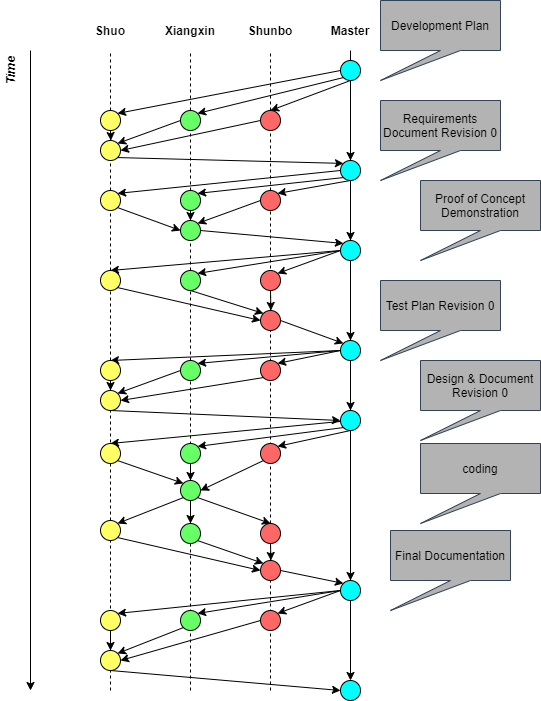
\includegraphics[width=12cm, height=16cm]{GitWorkFlow.png}
\section{Proof of Concept Demonstration Plan}
    The most challenging part in the implementation is the modification of the game complexity. The mechanism of original game is simple, since it only contains an empty map and a character controlled by the player. We will introduce a new operation mechanism to the game. The snake will stay at the center of the screen, while the map moves relative to the snake. To achieve this we need to modify the operation logic in the GameBoardPanel class. If the head of the snake remains at the center and the map is always able to move in the reverse direction of the player's input, the implementation is valid.\\
    Another feature being added to the game is the boosting item generation. This will also need to be implemented in the map class as an attribute for each map. As a result of consuming the items, the snake will gain temporary buff, which will be an additional attribute of the snake class. The function meets the requirement if the buff starts as the head of snake reaches the location of the item, and the buff ends automatically after some fixed time period. Java can support all these additional functions in less than 10 classes. \\
    The project is a light-weighted Java program and it does not require high performance of the personal computer. The only required library is Java which is available on most computer system. The game will be able to run on any computer with Java terminal so it has high capability. We will use JUnit for the testing of the game. The possible game events and operations will be covered in the test.
\section{Technology}
    \begin{enumerate}
        \item The whole project will be implemented in Java. Game functions including the game board panel, snake, input manager will be implemented in different modules.
        \item Eclipse will be used as IDE for the project.
        \item JUnit will be used for testing each modules.
        \item We will keep using LaTeX for the following documentations.
    \end{enumerate}
\section{Coding Style}
This project adapt the coding style similar to Oracle's Java code conventions. Each Java source file contains a single public class or interface. All source files should begin with copyright notice and a brief description of the purpose of the program. Only one declaration per line is encouraged. Never declare variables and functions or different types on the same line.Put declarations at the beginning of blocks rather than until their first use. For the naming converntion, all instance names are in mixed case with a lowercase first letter. Internal words start with capital letters. Constant name should be all uppercase with words separated by underscores “\_”.
\section{Project Schedule}

Provide a pointer to your Gantt Chart.
\href{run:./Milestone.pdf}{Milestone.pdf}

\section{Project Review}

\end{document}
